\section{RISMC Approach to Multi-Unit Modeling}
\label{sec:RISMC_MU_modeling}

The actual multi-unit model has been modeled using both RELAP5-3D and RAVEN.
The RELAP5-3D models are employed to determine the temporal response of all PWRs and SFPs while the plant 
connections and dependencies have been coded as an external model in RAVEN.
The connections between the RELAP5-3D models and the RAVEN plant model are 
shown in Fig.~\ref{fig:ensembleModel}.

The multi-unit model is structured so that it receives in input the set of 
sampled values (refer to Section~\ref{sec:plantStochasticModeling} for the complete list of 
the chosen stochastic parameters) and it provides in output the status of the six
models (PWRs and SFPs).
Internally, the multi-unit model consists of a plant model in series with the six 
RELAP5-3D models (which are arranged in a parallel configuration).
The plant model determines timing and sequencing of events of the accident scenario
and it provide these vales to the RELAP5-3D models.

Section~\ref{sec:systemModels} describes in detail the RELAP5-3D models for 
the SFPs and the PWRs while Section~\ref{sec:plantModel} describes the plant 
model.
 
\begin{figure}
    \centering
    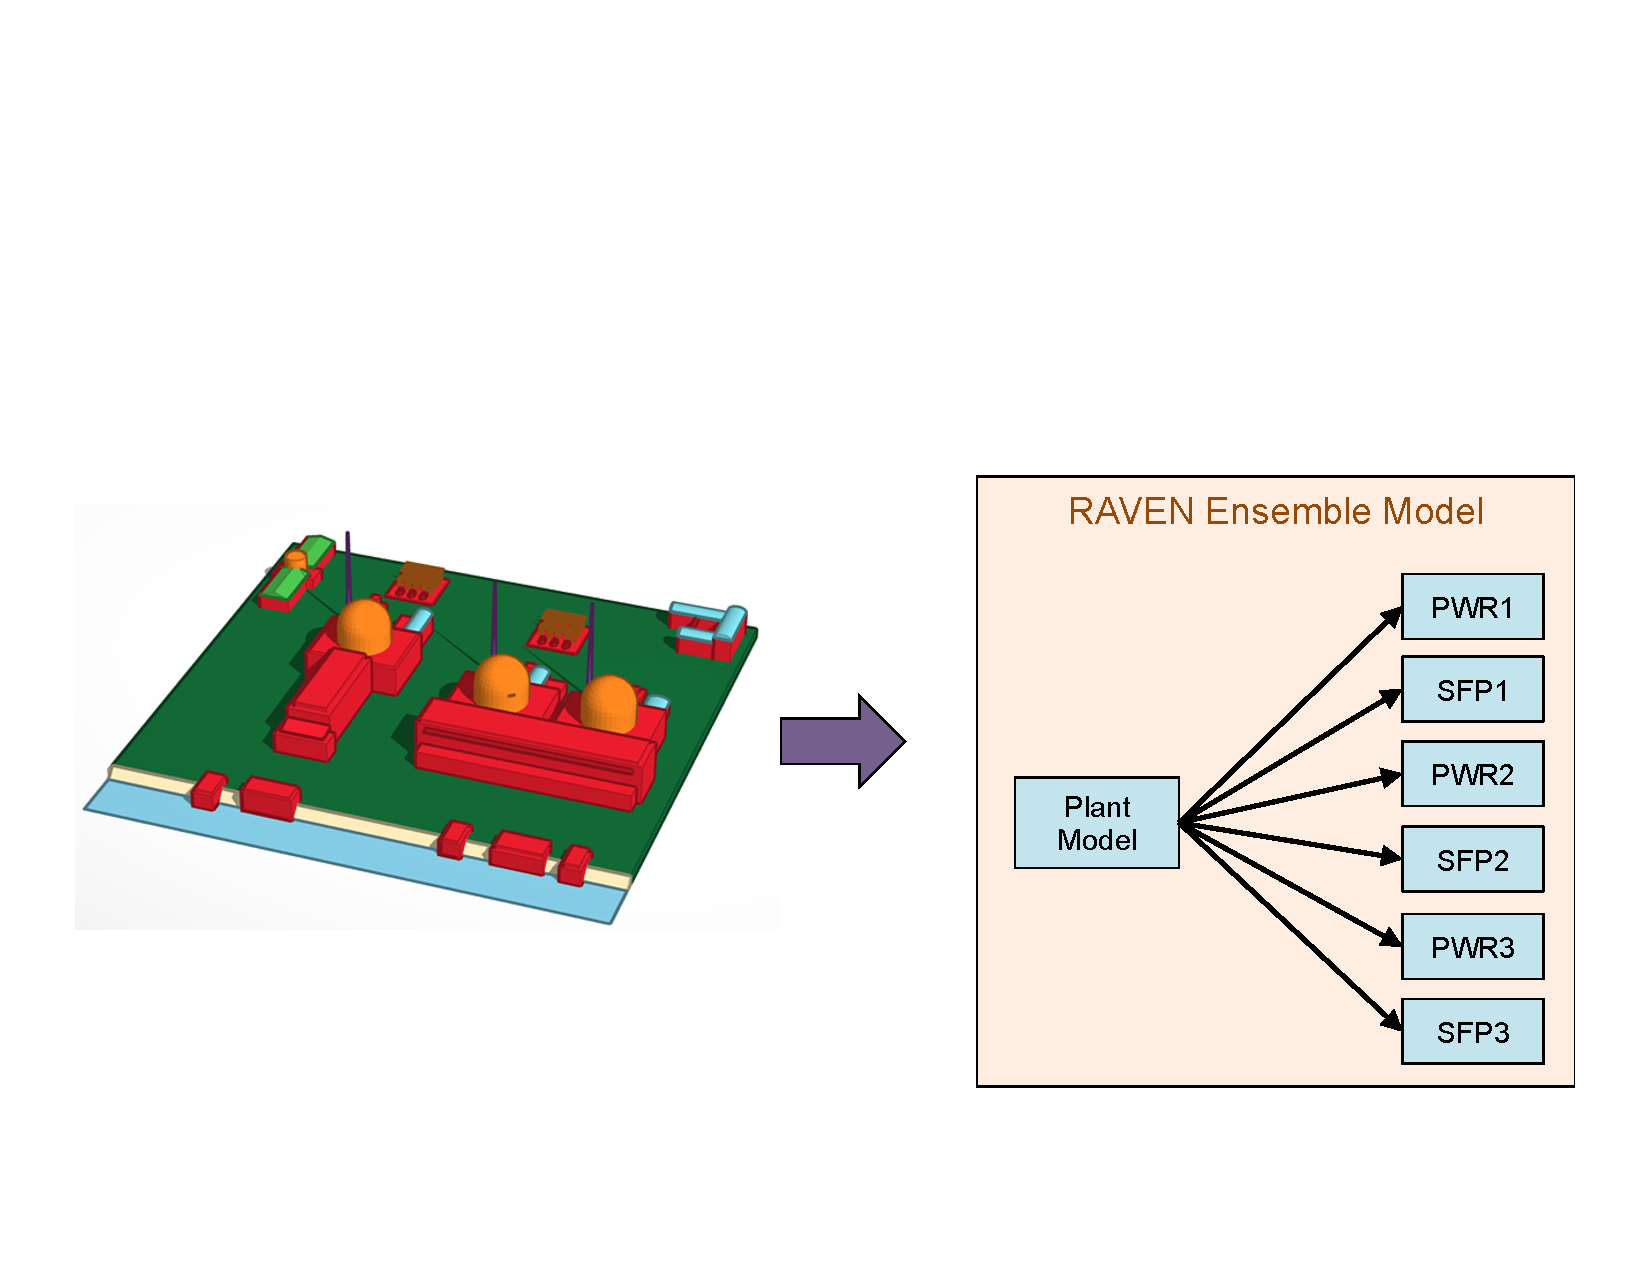
\includegraphics[scale=0.5]{ensembleModel.pdf}
    \caption{RAVEN ensemble model for the considered test case.}
    \label{fig:ensembleModel}
\end{figure}

\subsection{System Models}
\label{sec:systemModels}

\subsubsection{PWR1 and PWR3}
RELAP5-3D PWR models are based on the so-called INL Generic PWR (IGPWR) 
model~\cite{parisiExternalHazard,ronaldoRISMC}. 
The input deck is modeling a ~2.5 GWth Westinghouse 3-loop PWR, including the RPV,
the 3 loops and the primary and secondary sides of the steam 
generators (SGs) as shown in Fig.~\ref{fig:PWRnodalization}.
Four independent channels are used for representing the reactor core. Three channels model 
the active core and one channel models the core bypass. Different power values are assigned 
to the three core channels in order to take into account the radial power distribution. 
Passive and active heat structures simulate the heat transfer between the coolant and fuel, 
the structures and the secondary side of the IGPWR.
The possible operator actions that can occur during a SBO event with 
the reactor at full power (Unit 1 and Unit 3) are implemented through the RELAP5-3D control 
logic. These actions include SG cool-down, feed and bleed, AFW flow control, primary/secondary 
side emergency injection, etc.

\begin{figure}
    \centering
    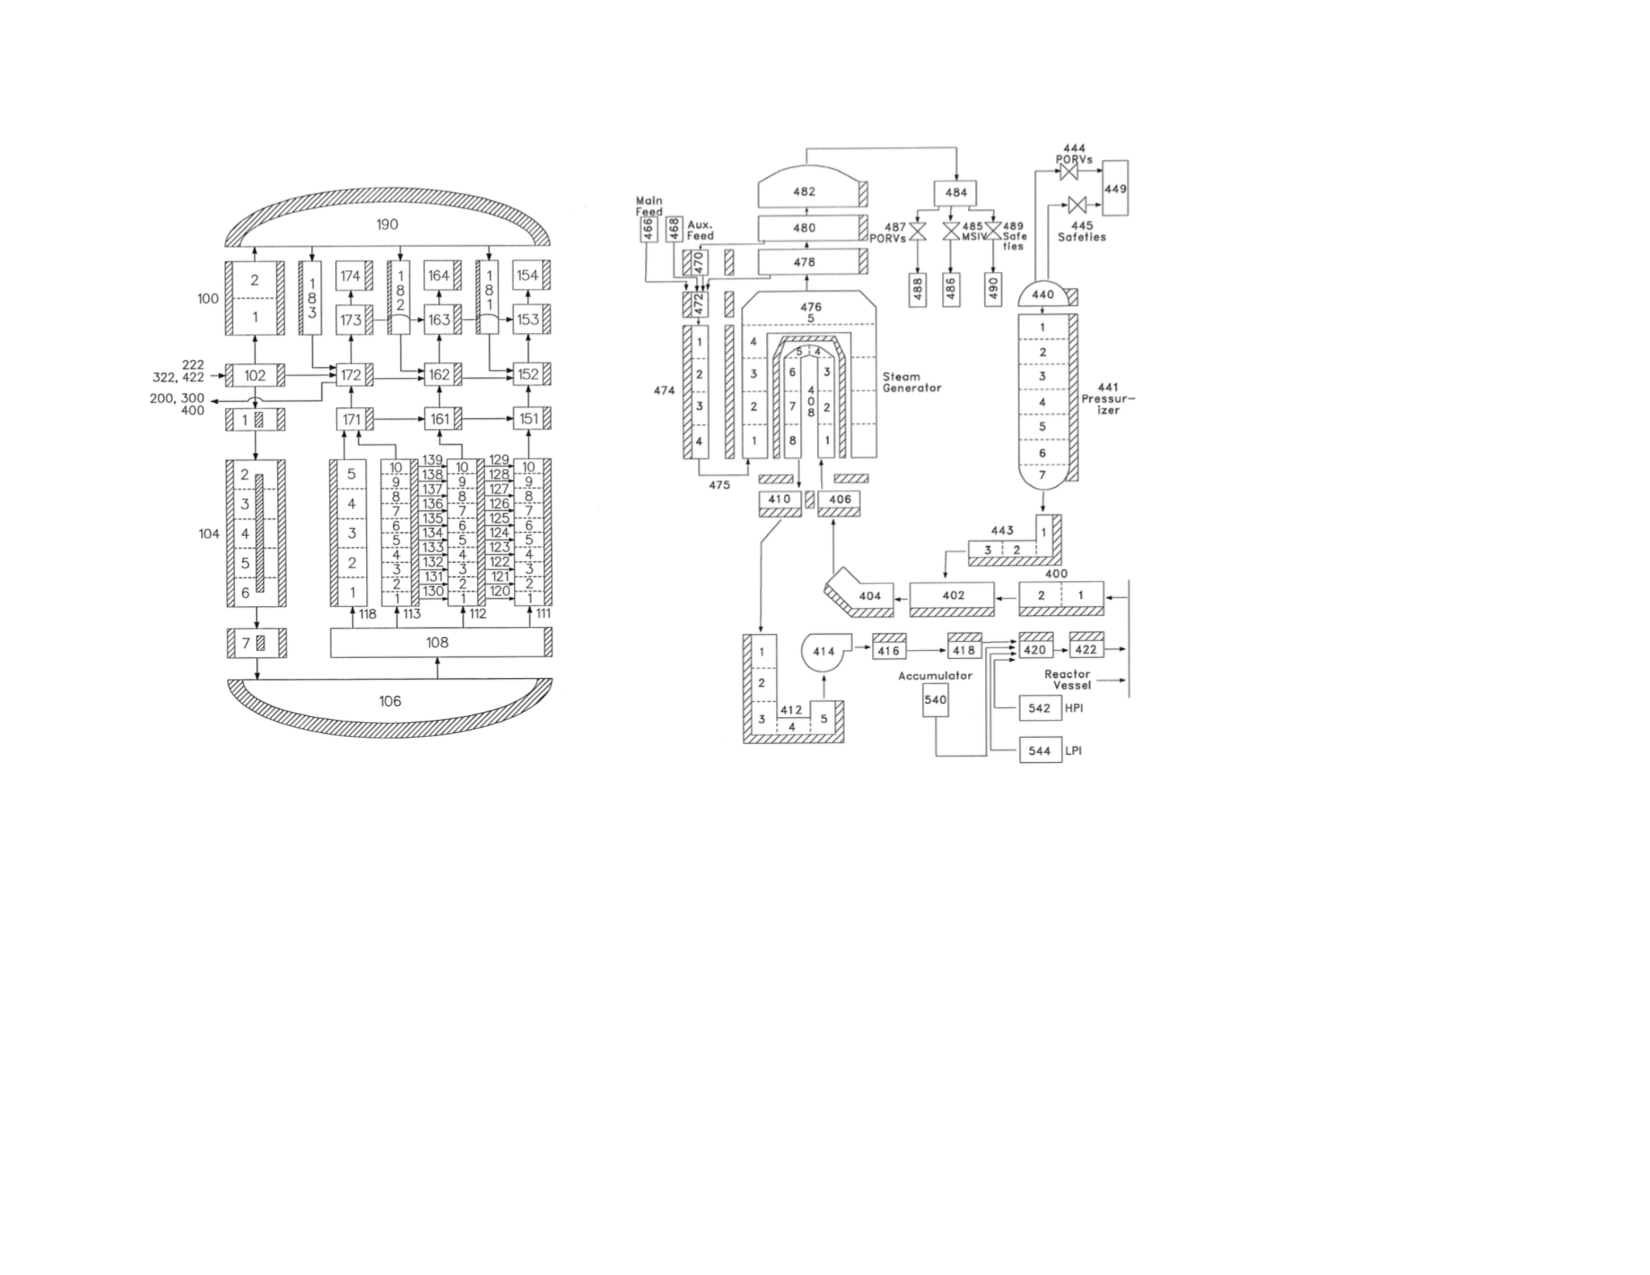
\includegraphics[scale=0.7]{nodalizationTMI.pdf}
    \caption{PWRs nodalization.}
    \label{fig:PWRnodalization}
\end{figure}

\subsubsection{PWR2}
Unit 2 is based on the same RELAP5-3D IGPWR model, consistently modified for simulating the 
mid-loop conditions~\cite{NUREGCR6144}. The model represents Unit 2 
during the refueling outage phase, with steam generator 3 manway opened for maintenance and pressurizer safety 
valves removed. Decay heat is removed by the Residual Heat Removal System (RHRS). Because the 
openings on the primary system (in the pressurizer and steam generator 3), the use of steam generators 
for reflux cooling in case 
of loss of RHR is prevented. However cooling by gravity drain from the RWST is possible.

The water level in the primary circuit is kept at the middle plane of the hot and cold legs 
by a recirculation circuit modeling the RHRS. 
The parts of the primary and the secondary systems with no water contain air at atmospheric condition.  
Main physical parameters values are reported in Table~\ref{tab:midLoopParamteres}.

\begin{table}
   \centering
   \begin{tabular}{|c|c|}
     \hline
     \textbf{Parameter}           & \textbf{Value}   \\ \hline \hline
     Core Power (MW)              & 13.0    \\ \hline
     RHR mass flow (kg/s)         & 235.0   \\ \hline
     RHR inlet temperature (K)    & 313     \\ \hline
     RHR outlet temperature (K)   & 327     \\ \hline
     Core average temperature (K) & 330     \\ \hline
  \end{tabular}
  \caption{Plant operating parameters at mid loop operation.}
  \label{tab:midLoopParamteres}
\end{table} 

\subsubsection{SFPs}
The three SFPs were also modeled~\cite{parisiExternalAnalysis} using RELAP5-3D. 
A scheme of a typical SFP is given in Fig.~\ref{fig:SFPnodalization}. 
For the sake of simplicity, the two cooling loops were modeled just as boundary conditions 
(assigned water inlet/outlet mass flow rates and temperatures). The opening of a valve on the pool bottom
could simulate the fuel pool break by seismic effects. The RELAP5-3D model is reported in Fig.~\ref{fig:SFPnodalization}.

The RELAP5-3D model was kept as simple as possible in order to reduce calculation times, e.g., 120 seconds 
of computer time was required for 86400 seconds transient. The thermal-hydraulic scheme is based on
43 volumes and 49 junctions. 2 Heat Structures are used for modeling $15 \times 15$ Westinghouse FA. 
The two independent cooling systems are modeled as boundary conditions (i.e., mass flow and 
temperature inlet are imposed). A couple of valves are used to model medium and large breaks of the pool bottom.

The following control logic is also implemented. The cooling systems pumps trip if: 
\begin{itemize}
  \item SFP liquid level lower than 0.1 m or
  \item SFP temperature greater than 349 K
\end{itemize}

Emergency crew action (emergency water injection) is assumed when both the recirculation pumps trip. 
The average time of action of the emergency crew is derived from human reliability analysis is assumed 
to be 30 minutes.

\begin{figure}
    \centering
    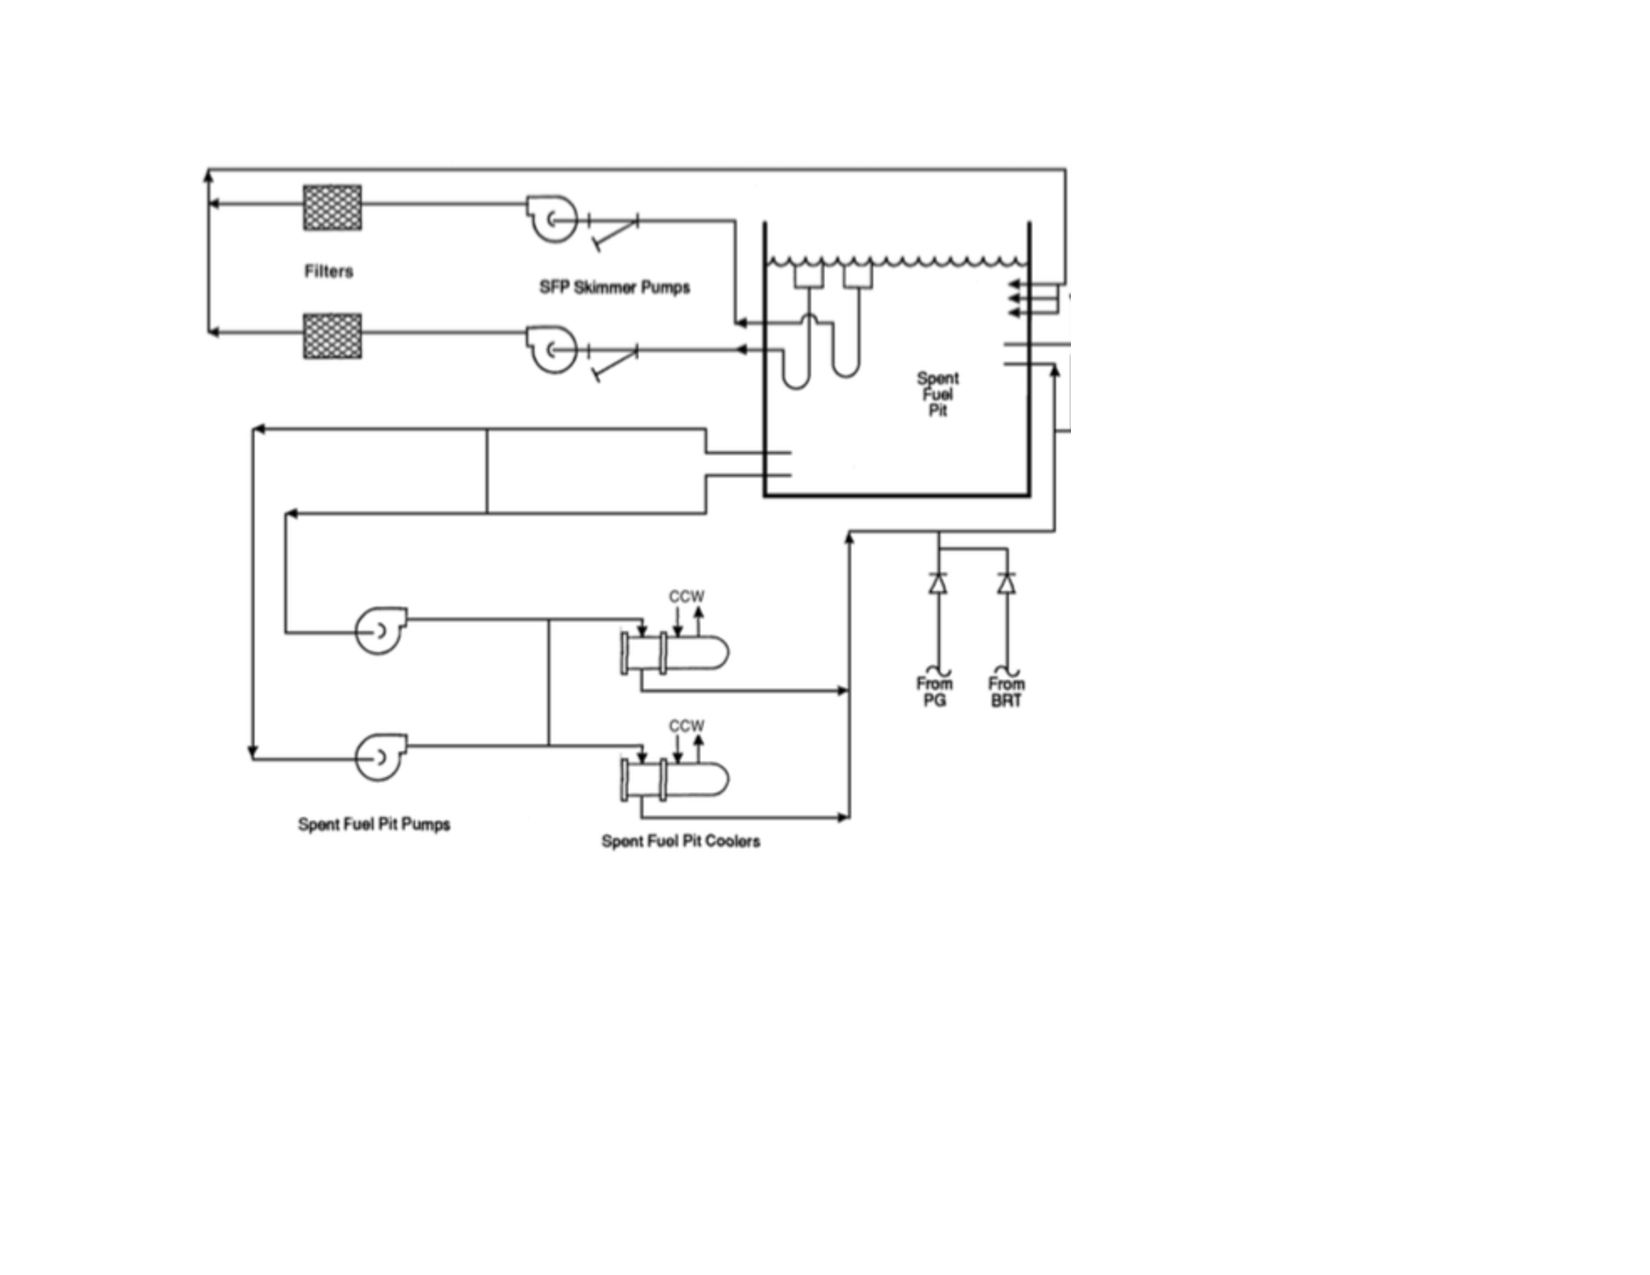
\includegraphics[scale=0.5]{nodalizationSFP.pdf}
    \caption{SFPs nodalization.}
    \label{fig:SFPnodalization}
\end{figure}

\subsection{Plant Model}
\label{sec:plantModel}
The plant model has been coded in Python script and interfaced with RAVEN as an 
external model. Its main purpose is to determine timing and sequencing of events 
for all six system models (i.e., PWRs and SFPs) given the sampled values of the 
stochastic parameters.

\subsection{Human Models}
To consider the performance of field workers, a simple human reliability analysis was 
performed and incorporated into the event simulation. Although many human actions are 
required, the analysis considers two human events: time to start recovery procedures 
after initiating event and EDGS erroneous alignment.

Regarding the first, we employed a detailed subtask modeling using the HUNTER~\cite{boringHUNTER} 
framework. The details about 
the model can be found in~\cite{hunterReport2016}; for the scope of this report, this event 
is modeled as a stochastic variable with a pdf derived from~\cite{hunterReport2016}. 

Regarding the second human related event, in order to screen the impact of the possible error, 
the human error probability 
(HEP) was obtained from the Technique for Human Error Rate Prediction (THERP) 
method~\cite{NUREGCR1278}. 
EDGS erroneous alignment corresponds well to THERP Table 20-13, Item 5: ``Making an error 
of selection in changing or restoring locally operated valve when the valve to be manipulated 
is unclearly or ambiguously labeled, part of a group of two or more valves that are similar in 
all of the following, size and shape, state, and presence of tags.'' This THERP item captures 
the nature of the task, particularly regarding complexity and ambiguity about pipe arrangements 
and corresponding valve operation. 

THERP produces an HEP equal to $1.0 \cdot 10^{-2}$, with an uncertainty 
error factor of 3. THERP includes provision for considering additional degradation of performance 
due to lack of experience and situational stress. These factors were not deemed likely contributors 
to the event outcome. Event recovery was not modeled.

Thus in the analysis, we have modeled erroneous alignment of EDGS with a Bernoulli 
distribution with value of $p=1.0 \cdot 10^{-2}$.

\subsection{Plant Stochastic Modeling}
\label{sec:plantStochasticModeling}
For the scope of this analysis, we have identified 23 stochastic parameters. We have 
grouped these parameters based on their area of interest.

Regarding the SFPs, we have have identified seismic induced rupture, i.e., a SFP Loss Of
Coolant Accident (LOCA), as 
element to include into the analysis. SFP LOCA has been represented by two stochastic 
parameters: time of occurrence and size of the SFP LOCA. In this work we have identified 
with locaTimeSFP1, locaTimeSFP2 and locaTimeSFP3 as the time of occurrence of the SFP 
LOCAs while locaSizeSFP1, locaSizeSFP2 and locaSizeSFP3 represents the actual size of 
the SFP LOCAs.

Regarding the PWRs, we selected two elements: lifetime of the batteries and the LOCA 
associated to the seal of the Reactor Coolant Pumps (RCPs). Battery systems provides 
DC power to I\&C systems 
of the PWRs such as the control of the Pilot Operated Relief Valves (PORVs).
DC systems are considered for only 
Unit 1 and Unit 3; since Unit 2 is in mid-loop operation mode, its DC systems are not 
considered.

For the EDGS, we have identified the following parameters: the probability to 
erroneous align the EDGS from Unit 2 to Unit 1, the time of occurrence of EDGS
erroneous alignment and time required to perform EDGS voluntary alignment.  

Each cross-tie, CST (between Unit 2 and Unit 3), AFW (between Unit 1 and Unit 3) 
and AC (between Unit 1 and Unit 2), has been considered in the analysis and, in 
particular, they have been modeled by assigning to each of them the time required 
to perform such cross-tie.

Regarding the recovery of each unit through the EPEs, we have modeled them by 
representing them with a single stochastic parameter which represents the
time to connect the EPE to its own unit.

Lastly, the recovery plan followed by the plant crew has been modeled using a single
parameter: recoveryStrategy (see Section~\ref{sec:accidentProgression}).

In addition to recovery strategy, we have given an additional degree of freedom on 
the actual procedure associated to the EPE for Unit 3. 
As indicated in Section~\ref{sec:EPEactions}, depending on the  recovery strategy, 
then the EPE connection on Unit 3 can be performed in different modes. 

A summary of the chosen stochastic parameters are listed in Table~\ref{tab:stochasticParameters1} 
along with their description and probabilistic distribution function.

\begin{table}
  \centering
  \begin{center}
      \begin{tabular}{ | l | p{5cm} | c | p{5cm} |}
        \hline
         \textbf{Parameter}          & \textbf{Description}                      & \textbf{Unit}   & \textbf{Distribution}                                         \\ \hline \hline
         AUXFWxtieTime      & Time to perform AFW cross-tie    & hour   & Uniform (lower bound=.5, upper bound=1.5)            \\ \hline
         CSTxtieTime        & Time to perform CST cross-tie    & hour   & Uniform (lower bound=.5, upper bound=1.5)            \\ \hline
         recoveryStrategy   & Recovery strategy to be followed & -      & Categorical(1,2,3) (p(1)=.3, p(2)=.3, p(3)=.4)       \\ \hline
         recovProcedTime    & Time to start plant recovery procedure    & hour        & Truncated normal (mean=1., sigma=.2, lower bound=.5, upper bound=1.5)       \\ \hline
         EPETime1           & Time to connect EPE to Unit 1    & hour   & Truncated normal (mean=2., sigma=.3, lower bound=1., upper bound=3.)   \\ \hline
         EPETime2           & Time to connect EPE to Unit 2    & hour   & Truncated normal (mean=2., sigma=.3, lower bound=1., upper bound=3.)   \\ \hline
         EPETime3           & Time to connect EPE to Unit 3    & hour   & Truncated normal (mean=2., sigma=.3, lower bound=1., upper bound=3.)   \\ \hline
         EDGSerrAlign     & Probability of occurrence for EDGS erroneous alignment & -      & Bernoulli (p=0.01)                               \\ \hline
         EDGSerrAlignTime & Time of occurrence for EDGS erroneous alignment        & -      & Uniform (lower bound=.0, upper bound=1.)       \\ \hline
         batteryTime1       & Battery life for Unit 1          & hour      & Triangular (lower bound=6., upper bound=8., peak=7.) \\ \hline
         batteryTime3       & Battery life for Unit 3          & hour      & Triangular (lower bound=6., upper bound=8., peak=7.) \\ \hline
         EDGSswitchTime     & Time required to change EDGS alignment       & hour  & Uniform (lower bound=.25, upper bound=.75)                  \\ 
        \hline
      \end{tabular}
  \end{center}
  \caption{Summary of the stochastic parameters chosen for the multi-unit analysis and their associated distribution.}
  \label{tab:stochasticParameters1}
\end{table}
\addtocounter{table}{-1}
\begin{table}
  \centering
  \begin{center}
      \begin{tabular}{ | l | p{5cm} | c | p{5cm} |}
        \hline
         \textbf{Parameter}          & \textbf{Description}                      & \textbf{Unit}   & \textbf{Distribution}                                         \\ \hline \hline
         ACxTieUnit12       & Time to perform AC cross-tie     & hour      & Uniform (lower bound=.5, upper bound=1.)             \\ \hline
         locaTimePWR1       & Time of occurrence for PWR1 seal LOCA & hour & Uniform (lower bound=.1667, upper bound=.25)         \\ \hline
         locaTimePWR3       & Time of occurrence for PWR3 seal LOCA & hour & Uniform (lower bound=.1667, upper bound=.25)         \\ \hline
         locaSizeSFP1       & LOCA size for SFP1               & gpm       & Categorical(0.0004,0.0035,0.056) (p(0.0004)=.85, p(0.0035)=.1, p(0.056)=.05)   \\ \hline
         locaSizeSFP2       & LOCA size for SFP1               & gpm       & Categorical(0.0004,0.0035,0.056) (p(0.0004)=.85, p(0.0035)=.1, p(0.056)=.05)   \\ \hline
         locaSizeSFP3       & LOCA size for SFP1               & gpm       & Categorical(0.0004,0.0035,0.056) (p(0.0004)=.85, p(0.0035)=.1, p(0.056)=.05)   \\ \hline    
         locaTimeSFP1       & Time of occurrence for SFP1 LOCA & hour      & Categorical(0.,.1667,.333,.5,24.) (p(0.)=.025, p(.1667)=.025, p(.333)=.025, p(.5)=.025, p(24.)=.9)  \\ \hline
         locaTimeSFP2       & Time of occurrence for SFP2 LOCA & hour      & Categorical(0.,.1667,.333,.5,24.) (p(0.)=.025, p(.1667)=.025, p(.333)=.025, p(.5)=.025, p(24.)=.9)  \\ \hline
         locaTimeSFP3       & Time of occurrence for SFP3 LOCA & hour      & Categorical(0.,.1667,.333,.5,24.) (p(0.)=.025, p(.1667)=.025, p(.333)=.025, p(.5)=.025, p(24.)=.9)  \\ \hline
         flex3Strategy13    & Type of EPE connection for Unit 3 during recovery strategy 1 and 3  & -      & Categorical(1,2) (p(1)=.3, p(2)=.7)             \\ \hline
         flex3Strategy2     & Type of EPE connection for Unit 3 during recovery strategy 2        & -      & Categorical(1,2) (p(1)=.4, p(2)=.6)             \\ 
        \hline
      \end{tabular}
  \end{center}
  \caption{Summary of the stochastic parameters chosen for the multi-unit analysis and their associated distribution (cont.ed).}
  \label{tab:stochasticParameters2}
\end{table}


